% ============================================================================
%  PhD Thesis Skeleton — Chemistry (Indian University Standard)
%  Compile: pdflatex thesis && bibtex thesis && pdflatex thesis && pdflatex thesis
%  Structure per docs/03-thesis-blueprint.md:
%  preliminaries -> chapters 1..7 -> bibliography -> appendices
% ============================================================================
\documentclass[12pt,a4paper,oneside]{book}

\usepackage[utf8]{inputenc}
\usepackage[T1]{fontenc}
\usepackage{newtxtext,newtxmath}

% --- Layout: A4, 1.5in left (binding), 1in others, 1.5 line spacing ---
\usepackage[a4paper,left=1.5in,right=1in,top=1in,bottom=1in]{geometry}
\usepackage{setspace}
\onehalfspacing

% --- Chemistry ---
\usepackage[version=4]{mhchem}
\usepackage{chemfig}
\usepackage{siunitx}

% --- Figures & tables ---
\usepackage{graphicx}
\graphicspath{{figures/}{chapters/figures/}}
\usepackage{booktabs,array,multirow}
\usepackage[font=small,labelfont=bf]{caption}
\usepackage{subcaption}
\usepackage{chemscheme}   % 'scheme' float environment for reaction schemes

% --- References (ACS numbered style typical for chemistry theses) ---
\usepackage[numbers,sort&compress]{natbib}
\bibliographystyle{unsrtnat}   % or: acs, rsc (via texlive-science)

% --- Hyperlinks, TOC depth ---
\usepackage[colorlinks=true,linkcolor=blue,citecolor=blue,urlcolor=blue]{hyperref}
\setcounter{tocdepth}{3}
\setcounter{secnumdepth}{3}

% --- Page numbering: roman prelims, arabic body ---
\usepackage{afterpage}

\title{Thesis Title:\\Subtitle}
\author{Candidate Name\\Indian Institute of Science Education and Research Bhopal}

\begin{document}

% ============================================================================
% PRELIMINARY PAGES
% ============================================================================
\frontmatter
\pagenumbering{roman}

% ============================================================================
% Preliminary pages: title page, certificate, declaration, acknowledgements,
% abstract. ADAPT WORDING AND LOGO PLACEMENT TO YOUR INSTITUTE'S MANUAL.
% ============================================================================

% --- Title page (counted as page i, not printed) ---
\begin{titlepage}
\begin{center}
\vspace*{1cm}
{\Large \textbf{Thesis Title:\\Subtitle}}\\[1.5cm]
{\large A thesis submitted in partial fulfilment of the requirements\\ for the degree of \textbf{Doctor of Philosophy}}\\[1.5cm]
{\large by}\\[0.5cm]
{\Large \textbf{Candidate Name}}\\[0.3cm]
{\large (Roll Number: XXX})\\[1.5cm]
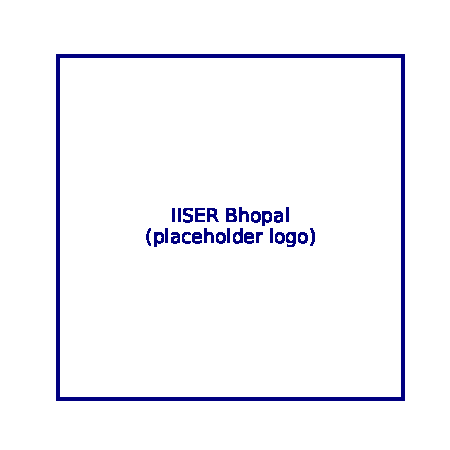
\includegraphics[width=3cm]{iiserb_logo.pdf}\\[1cm]
{\large Department of Chemistry}\\
{\large Indian Institute of Science Education and Research Bhopal}\\
{\large Bhopal Bypass Road, Bhauri, Bhopal 462066, Madhya Pradesh, India}\\[1cm]
{\large \the\year}
\end{center}
\end{titlepage}

% --- Supervisor's certificate ---
\chapter*{Certificate}
\addcontentsline{toc}{chapter}{Certificate}
\thispagestyle{empty}
This is to certify that the thesis entitled \emph{``Thesis Title''} submitted by
\textbf{Candidate Name} (Roll No. XXX) to the Indian Institute of Science
Education and Research Bhopal for the award of the degree of \textbf{Doctor of
Philosophy} is a record of bona fide research work carried out by him/her under
my supervision. The work has not been submitted elsewhere for any other degree.

\vspace{2cm}
\begin{flushright}
\textbf{Supervisor Name}\\
Professor, Department of Chemistry\\
IISER Bhopal\\[0.5cm]
Date:
\end{flushright}

% --- Candidate's declaration ---
\chapter*{Declaration}
\addcontentsline{toc}{chapter}{Declaration}
\thispagestyle{empty}
I declare that the thesis entitled \emph{``Thesis Title''} submitted by me for
the award of the degree of \textbf{Doctor of Philosophy} is a record of work
carried out by me under the supervision of Prof.~Supervisor Name. The work is
original and has not been submitted, in part or full, for any other degree or
diploma to this or any other institute/university. I further declare that the
thesis has been checked for plagiarism using [institute tool] and the similarity
index is within the permissible limit.

\vspace{2cm}
\begin{flushright}
\textbf{Candidate Name}\\
Department of Chemistry, IISER Bhopal\\[0.5cm]
Date:
\end{flushright}

% --- Acknowledgements ---
\chapter*{Acknowledgements}
\addcontentsline{toc}{chapter}{Acknowledgements}
\thispagestyle{empty}
I express my deepest gratitude to my supervisor, Prof.~Supervisor Name, for
\ldots{} I thank my doctoral committee members \ldots{} I am grateful to the
Central Instrumentation Facility, IISER Bhopal, for \ldots{} I thank my
collaborators \ldots{} Financial support from [Funding Agency, Grant No.] is
gratefully acknowledged. Finally, I thank my family and friends for \ldots{}

% --- Abstract ---
\chapter*{Abstract}
\addcontentsline{toc}{chapter}{Abstract}
\thispagestyle{empty}
(250--350 words; the four-move structure from docs/02: context, gap/approach,
key results with numbers, significance.)
          % title page, certificate, declaration, acknowledgements, abstract
\tableofcontents
\listoffigures
\listoftables
% Abbreviations & symbols list — make it chemistry-complete.
\chapter*{List of Abbreviations and Symbols}
\addcontentsline{toc}{chapter}{List of Abbreviations and Symbols}
\begin{tabular}{ll}
\textbf{1D/2D} & one-/two-dimensional \\
\textbf{Ac} & acetyl \\
\textbf{ACN / MeCN} & acetonitrile \\
\textbf{AIE} & aggregation-induced emission \\
\textbf{Ar} & aryl \\
\textbf{B3LYP} & Becke, 3-parameter, Lee--Yang--Parr (DFT functional) \\
\textbf{bpy} & 2,2$'$-bipyridine \\
\textbf{calc. / found} & calculated / found \\
\textbf{CCDC} & Cambridge Crystallographic Data Centre \\
\textbf{CDCl$_3$} & deuterated chloroform \\
\textbf{CIF} & Crystallographic Information File \\
\textbf{CV} & cyclic voltammetry \\
\textbf{DFT} & density functional theory \\
\textbf{DMSO} & dimethyl sulfoxide \\
\textbf{equiv.} & equivalent(s) \\
\textbf{ESI} & electrospray ionisation \\
\textbf{EtOAc} & ethyl acetate \\
\textbf{HRMS} & high-resolution mass spectrometry \\
\textbf{IR} & infrared \\
\textbf{J} & coupling constant (Hz) \\
\textbf{Me} & methyl \\
\textbf{mp} & melting point \\
\textbf{NMR} & nuclear magnetic resonance \\
\textbf{ORTEP} & Oak Ridge thermal ellipsoid plot \\
\textbf{PCM} & polarisable continuum model \\
\textbf{Ph} & phenyl \\
\textbf{rt} & room temperature \\
\textbf{SHELX} & structure solution/refinement program \\
\textbf{TMS} & tetramethylsilane \\
\textbf{UV--vis} & ultraviolet--visible \\
$\delta$ & chemical shift (ppm) \\
$\lambda$ & wavelength (nm) \\
$\Phi$ & quantum yield \\
$\tau$ & lifetime (ns) \\
$\tilde{\nu}$ & wavenumber (cm$^{-1}$) \\
\end{tabular}
    % list of abbreviations & symbols

% ============================================================================
% MAIN BODY
% ============================================================================
\mainmatter
\pagenumbering{arabic}

% ============================================================================
% Chapter 1 — Introduction and Literature Review
% Guidance: docs/03-thesis-blueprint.md section 2.
% ============================================================================
\chapter{Introduction and Literature Review}
\label{ch:intro}

\section{Background and motivation}
\label{sec:background}
The broader field context \ldots{} (cite seminal reviews).

\section{Literature review}
\label{sec:litrev}
\subsection{Theme one: ...}
\label{sec:theme1}
\ldots{} organised thematically, each subsection ending with the open question
that this thesis addresses. Include the most recent 3--5 years of work.

\subsection{Theme two: ...}
\label{sec:theme2}
\ldots{}

\section{Knowledge gap and objectives}
\label{sec:gap}
Despite the progress summarised above, \ldots{} remains unexplored
\citep{keyref2023}. This thesis addresses this gap with the following
objectives:
\begin{enumerate}
  \item Objective one;
  \item Objective two;
  \item Objective three.
\end{enumerate}

\section{Organisation of the thesis}
\label{sec:org}
Chapter 2 describes materials and methods \ldots{} Chapters 3--5 present the
results \ldots{} Chapter 6 summarises conclusions and future directions.

% ============================================================================
% Chapter 2 — Materials and Methods (shared general methods)
% ============================================================================
\chapter{Materials and Methods}
\label{ch:methods}

\section{Reagents and solvents}
\label{sec:reagents}
All reagents were purchased from commercial suppliers and used as received
unless otherwise stated. Dry solvents (THF, DCM, toluene) were obtained from a
solvent purification system. Column chromatography was performed on silica gel
(100--200 mesh).

\section{Instrumentation}
\label{sec:instruments}
NMR: Bruker Avance \SI{400}{\mega\hertz} and \SI{500}{\mega\hertz}
spectrometers; chemical shifts in ppm relative to TMS; coupling constants in Hz.
HRMS: Bruker microTOF-Q II (ESI). IR: PerkinElmer Spectrum Two (ATR). UV--vis:
Shimadzu UV-2600. Fluorescence: Horiba Fluorolog-3. SCXRD: Bruker D8 Venture.
CV: CH Instruments 600E. Computational: Gaussian 16 / ORCA 5.0.

\section{General experimental procedures}
\label{sec:genproc}
\subsection{Standard characterisation protocol}
\label{sec:charproto}
Every new compound was characterised by \ce{^1H} and \ce{^{13}C}\{\ce{^1H}\} NMR,
HRMS, IR and melting point; purity was confirmed by elemental analysis where
required. Crystals suitable for SCXRD were deposited at the CCDC (numbers
quoted per chapter); checkCIF reports are compiled in Appendix A.

\section{Computational methods}
\label{sec:compmethods}
Geometry optimisations were performed at the \texttt{PBE0-D3BJ/def2-TZVP} level
using Gaussian 16 (Revision C.01). Solvation effects were included via the
IEFPCM model (THF). All stationary points were verified by frequency analysis.
Coordinates are listed in Appendix C.

% ============================================================================
% Chapter 3 — Results: Story A (paper-shaped unit)
% Pattern for all results chapters: chapter intro -> results -> summary.
% ============================================================================
\chapter{Results: [Title of Story A]}
\label{ch:resultsA}

\section{Introduction to this study}
\label{sec:resA-intro}
Brief chapter-specific background (1--2 pages) recapping only what this chapter
needs \citep{keyref2021}. Parts of this chapter are published: \citep{mypub2024}.

\section{Synthesis}
\label{sec:resA-synth}
\ldots{} Scheme~\ref{sch:3-1} summarises the route.

\begin{scheme}[htbp]
\centering
\schemestart
\chemfig{A-B}
\arrow{->[conditions][yield]}
\chemfig{C-D}
\schemestop
\caption{Synthetic route.}
\label{sch:3-1}
\end{scheme}

\section{Characterisation}
\label{sec:resA-char}
\ldots{} Figure~\ref{fig:3-1}. Crystallographic confirmation: compound \textbf{8}
crystallises in $P2_1/c$ \ldots{} (CCDC 2400001).

\begin{figure}[htbp]
\centering
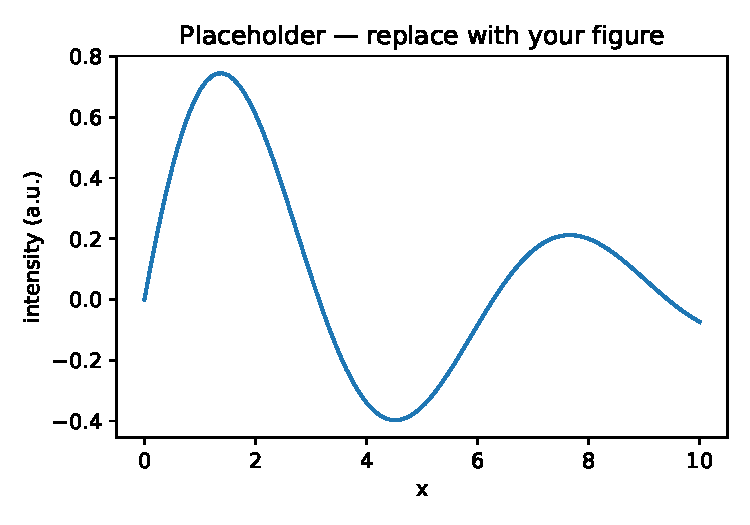
\includegraphics[width=0.8\linewidth]{fig31.pdf}
\caption{Key characterisation: X-ray structure / spectra / plot.}
\label{fig:3-1}
\end{figure}

\section{Discussion}
\label{sec:resA-disc}
\ldots{}

\section{Chapter summary}
\label{sec:resA-sum}
In this chapter, we demonstrated \ldots{} (3--5 sentences with data).

% ============================================================================
% Chapters 4 & 5 — Results: Stories B and C (duplicate the ch3 pattern)
% ============================================================================
\chapter{Results: [Title of Story B]}
\label{ch:resultsB}

\section{Introduction to this study}
\label{sec:resB-intro}
\ldots{}

\section{Results}
\label{sec:resB-results}
\ldots{}

\section{Discussion}
\label{sec:resB-disc}
\ldots{}

\section{Chapter summary}
\label{sec:resB-sum}
\ldots{}

% ============================================================================
% Chapter 5 — Results: Story C (duplicate the ch3 pattern)
% ============================================================================
\chapter{Results: [Title of Story C]}
\label{ch:resultsC}

\section{Introduction to this study}
\label{sec:resC-intro}
\ldots{}

\section{Results}
\label{sec:resC-results}
\ldots{}

\section{Discussion}
\label{sec:resC-disc}
\ldots{}

\section{Chapter summary}
\label{sec:resC-sum}
\ldots{}

% ============================================================================
% Chapter 6 — Conclusions and Future Directions
% ============================================================================
\chapter{Conclusions and Future Directions}
\label{ch:conclusions}

\section{Conclusions}
\label{sec:concl}
The work presented in this thesis led to the following conclusions:
\begin{enumerate}
  \item \textbf{[Conclusion 1 with data]}: \ldots{}
  \item \textbf{[Conclusion 2 with data]}: \ldots{}
  \item \textbf{[Conclusion 3 with data]}: \ldots{}
\end{enumerate}

\section{Limitations}
\label{sec:limits}
The present study is limited by \ldots{} (be honest; examiners reward it).

\section{Future directions}
\label{sec:future}
\begin{enumerate}
  \item Concrete idea one (with preliminary reasoning);
  \item Concrete idea two;
  \item Concrete idea three.
\end{enumerate}


% ============================================================================
% BACK MATTER
% ============================================================================
\backmatter
\bibliography{thesis}

\appendix
% ============================================================================
% Appendices: spectra compilation, list of publications.
% ============================================================================
\chapter{Spectra Compilation}
\label{app:spectra}
All \ce{^1H} and \ce{^{13}C} NMR spectra of new compounds are reproduced on the
following pages (one compound per page, structure inset).

% One page per compound:
\clearpage
\begin{figure}[htbp]
\centering
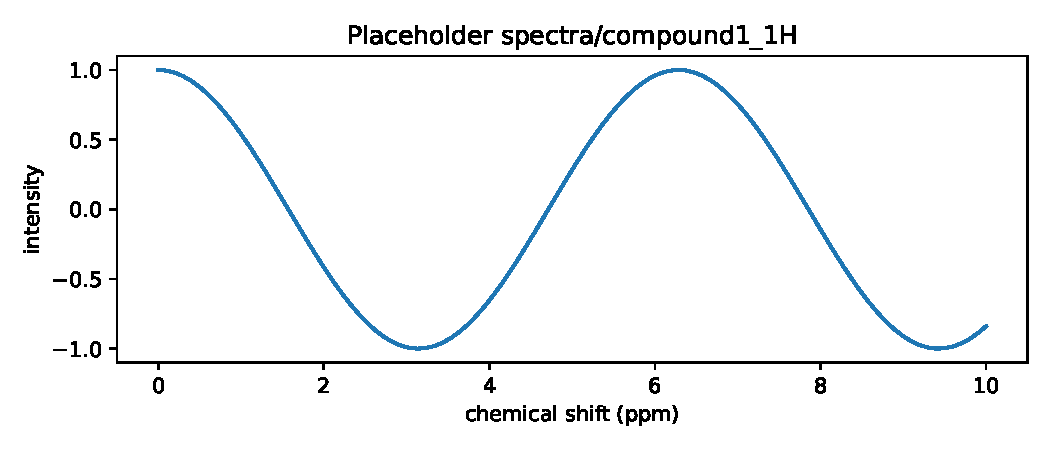
\includegraphics[width=0.95\linewidth]{spectra/compound1_1H.pdf}\\
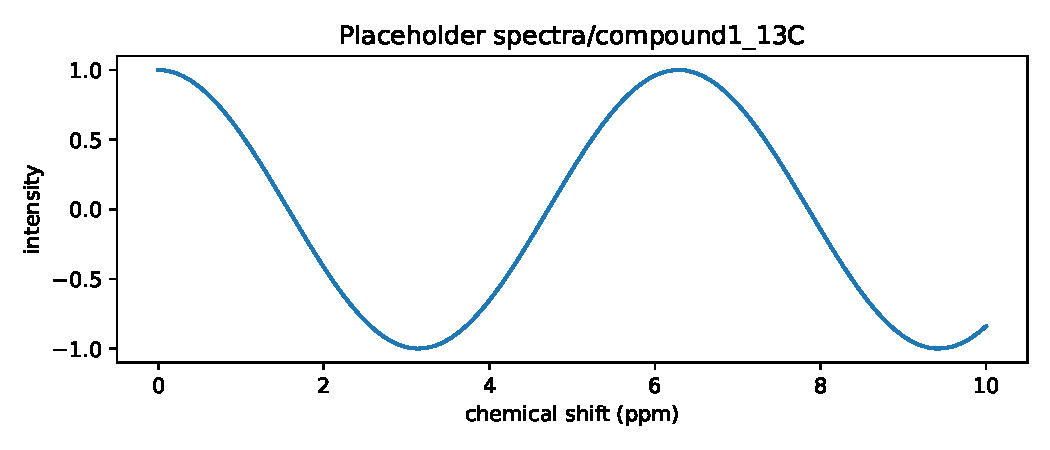
\includegraphics[width=0.95\linewidth]{spectra/compound1_13C.pdf}
\caption{\ce{^1H} and \ce{^{13}C} NMR spectra of compound \textbf{1}
(\SI{400}{\mega\hertz}, \ce{CDCl3}).}
\end{figure}

% ============================================================================
% Appendix: list of publications arising from the thesis work.
% ============================================================================
\chapter{List of Publications and Presentations}
\label{app:pubs}

\section{Publications from thesis work}
\begin{enumerate}
  \item Candidate, A.; Supervisor, B.; Coauthor, C. Title one. \emph{Journal} \textbf{Year}, \emph{Volume}, pages. DOI.
  \item Candidate, A.; Supervisor, B. Title two. \emph{Journal} \textbf{Year}, \emph{Volume}, pages. DOI.
\end{enumerate}

\section{Other publications}
\begin{enumerate}
  \item \ldots{}
\end{enumerate}

\section{Conference presentations}
\begin{enumerate}
  \item ``Talk/poster title'', Conference name, Place, Year.
\end{enumerate}


\end{document}
